\item

Durch identisches Umformen erhalten wir:

$$y'(y-2) = 3-x$$
$$\implies y' = \frac{3-x}{y-2}$$

Für diese DGL können wir das Richtungsfeld von einem Rechner zeichnen lassen. Um eine partikuläre Lösung zu finden, starten wir an dem gegebenen Anfangspunkt und folgen den Richtungspfeilen. Es ergeben sich Kreise mit dem Ursprung $(3, 2)$ als Lösungskurven der DGL.

Das Online-Tool verwendet sogenannte numerische Lösungsverfahren, welche die wahre Lösungsfunktion aufgrund der Beschränktheit der Gleitkommazahlen nur approximativ (näherungsweise) ermitteln können. Ein einfaches solches Näherungsverfahren besteht darin, vom durch den Anfangswert gegebenen Punkt auszugehen (vgl. Abbildung \ref{ex-ode-slope-field-1-img-b}). In finiten Schritten $\Delta x$ wird dann entsprechend dem momentanten Anstieg nach links bzw. nach rechts geschritten. Wo die Sprünge zu sehen sind, ist der Betrag des Anstiegs $|y'|$ sehr groß, sodass auch der Fehler bei einem Schritt $\Delta x$ groß wird. Am linken bzw. rechten Punkt des Kreises ist der Anstieg nicht mehr endlich.

\begin{figure}[ht]
	\centering
	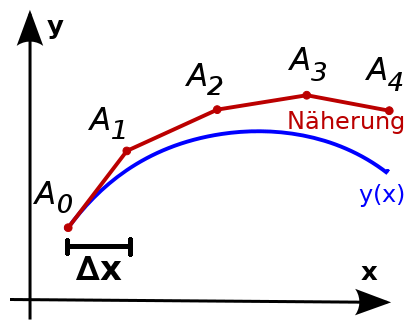
\includegraphics[width=0.4\textwidth]{../tex-snippets/ex-ode-slope-field-1-img-b.png}
	\caption{Einfaches numerisches Lösungsverfahren einer DGL der Ordnung 1 (Eulerverfahren). Es wird in endlich Schritten $\Delta x$ mit dem jeweiligen Anstieg von $A_0$ nach rechts zu $A_4$ geschritten. Die so erhaltene Kurve (rot) weicht von der tatsächlichen Lösungskurve (blau) ab. Je größer der Anstieg der Lösungskurve, desto größer ist der (absolute) Fehler bei gegebenem $\Delta x$.}
	\label{ex-ode-slope-field-1-img-b}
\end{figure}

